\documentclass[11pt,a4paper]{article}
\usepackage[utf8]{inputenc}
\usepackage{amsmath}
\usepackage{amsfonts}
\usepackage{amssymb}
\usepackage{graphicx}
\usepackage{verbatim}
\usepackage{float}

\author{Jan Kramer\\Klaas Kliffen}
\title{Computervision Lab 1}
\begin{document}
\maketitle

\section*{Exercise 1}

\begin{figure}[h]
\centering
    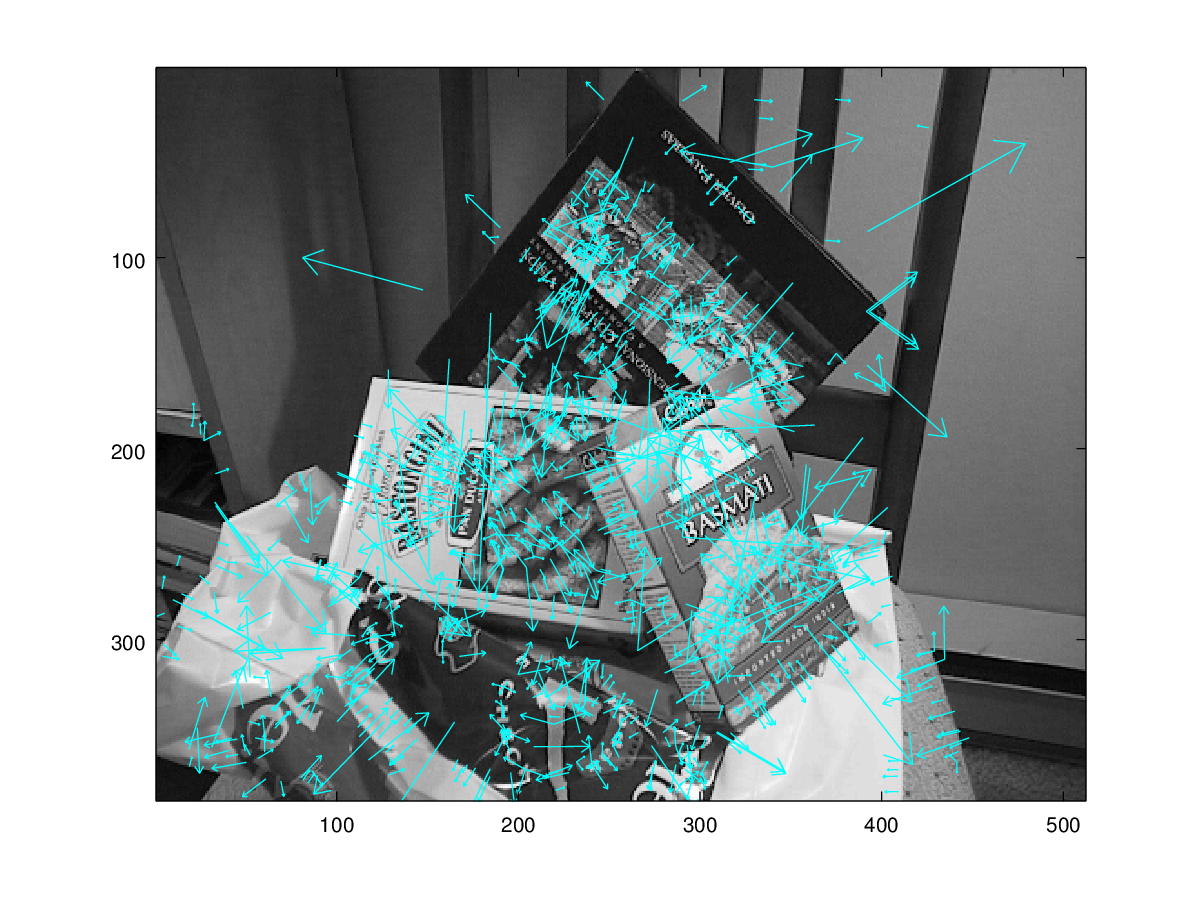
\includegraphics[width=0.9\textwidth]{./img/scene-keys.png} \\
\caption{The features SIFT finds in ``scene.pgm"}
\label{fig:scenekeys}
\end{figure}

The features SIFT finds in ``scene.pgm" are shown in Figure \ref{fig:scenekeys}.
Since SIFT uses the differences of gaussian pyramid technique, most keys can be found in regions where the intensities change.
These regions can be small or large depending on where in the pyramid it was found.
Running the \verb+whos+ command gives us the number of keys that are shown in this image, namely 1021 keys with 128 elements.
The SIFT paper mentions that the number of expected keys is in the order of thousands for a 512 by 512 pixel image.
Since our image is only 512 by 384 pixels, we can expect less.
Hence the number that we found is probably in agreement with the paper.
Also note that the number of elements in the keys are different from the paper, keys in the paper have 160 instead of 128 elements.
We assume the cause is that this implementation does not sample a higher plane in the image pyramid, since the difference in number of elements is in agreement with the number of samples taken in this plane.

\begin{figure}
\centering
    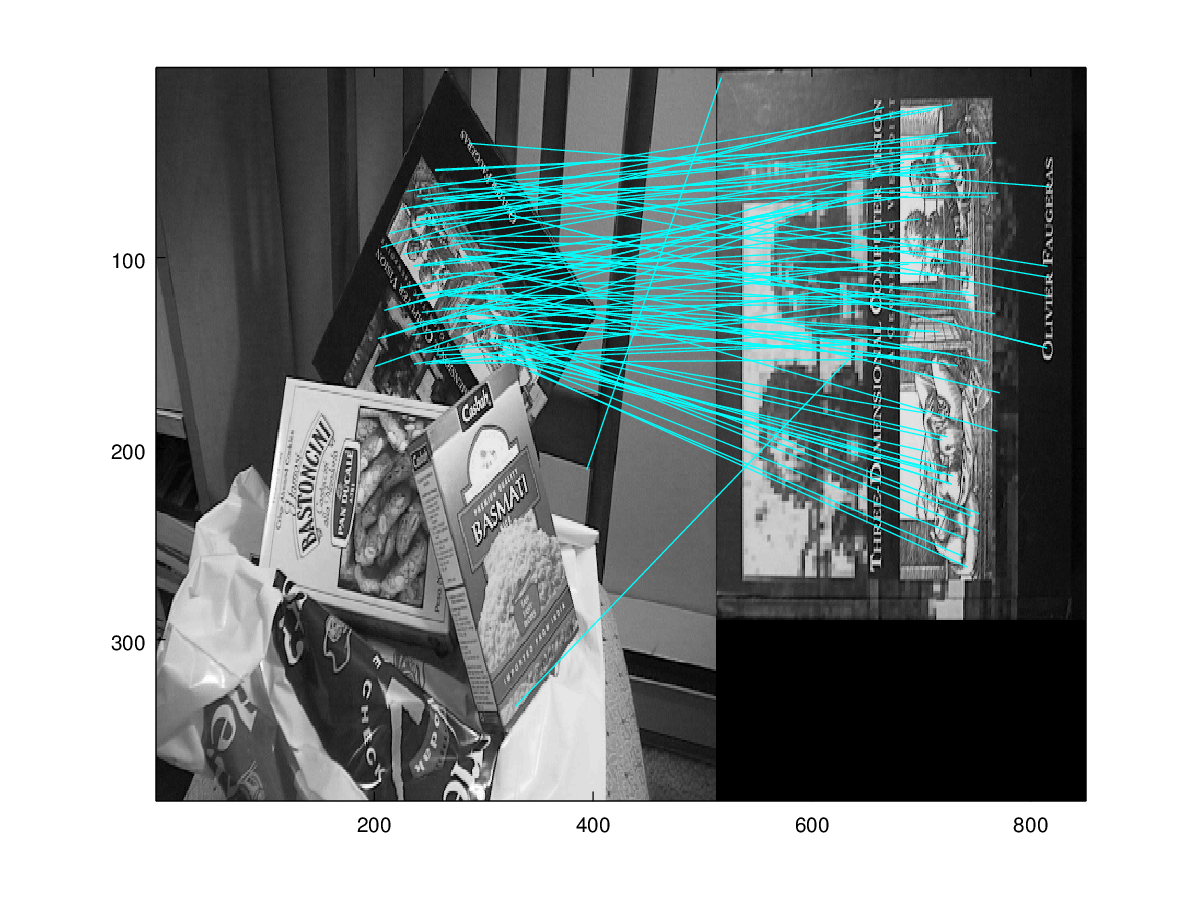
\includegraphics[width=0.9\textwidth]{./img/scene-book-match.png} \\
\caption{The matching features SIFT finds in ``scene.pgm" with ``book.pgm"}
\label{fig:scenebookmatch}
\end{figure}

The result of matching this scene with ``book.pgm" is shown in Figure \ref{fig:scenebookmatch}, it also shows the 98 matching keypoints with lines denoting matches.
This amounts to $9.5\%$ of the keypoints in ``scene.pgm" and $11\%$ of the keypoints in ``book.pgm".
It also shows two mismatches.
The first mismatch is between a corner from the book and a corner in the background of the scene.
The second one is between part of the bowl of rice and part of the image of the book.
It is understandable that these matches exist, since the features(colors/texture) are similar in the neighborhoods of the keypoints if you account for orientation.

\begin{figure}
\centering
    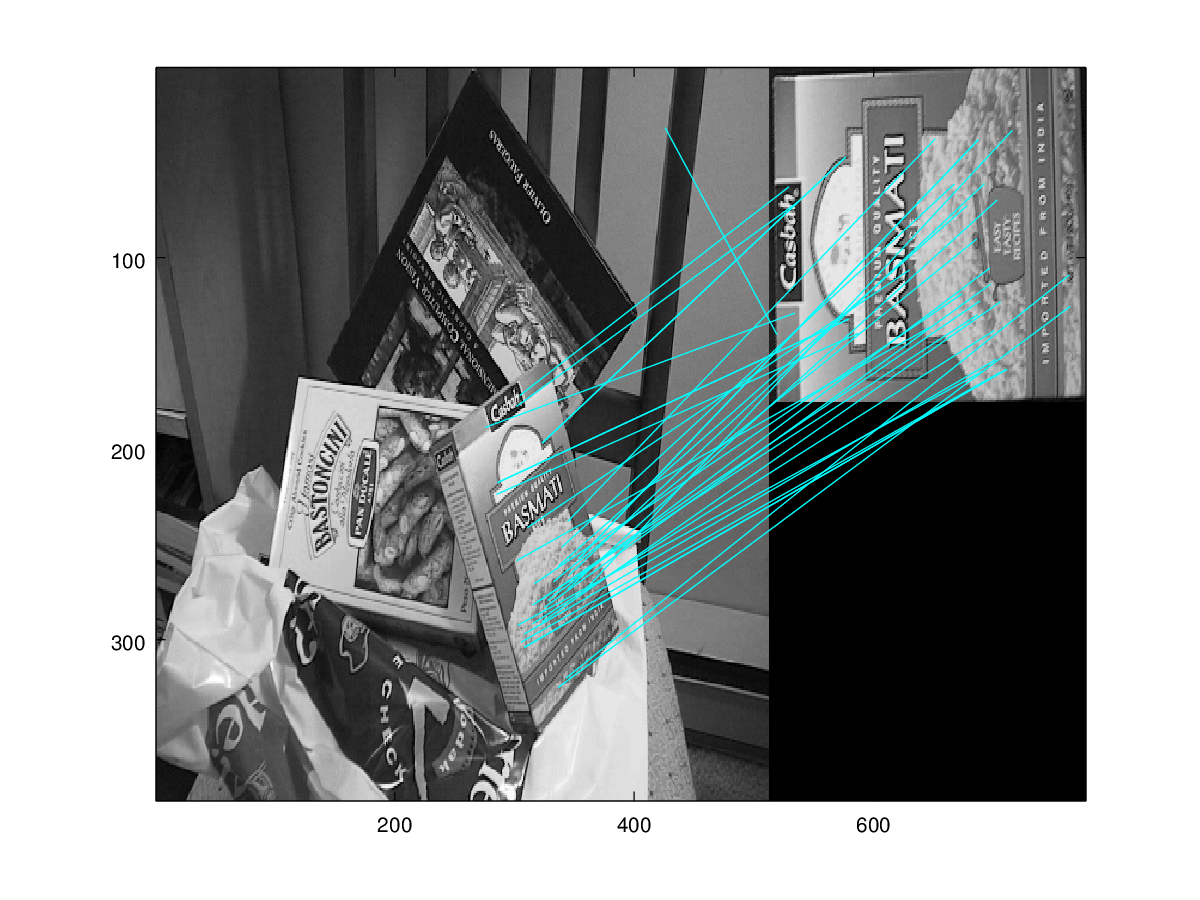
\includegraphics[width=0.9\textwidth]{./img/scene-basmati-match.png} \\
\caption{The matching features SIFT finds in ``scene.pgm" with ``basmati.pgm"}
\label{fig:scenebasmatimatch}
\end{figure}

The result of matching this scene with ``basmati.pgm" is shown in Figure \ref{fig:scenebasmatimatch}, it also shows the 34 matching keypoints with lines denoting matches.
This amounts to $3.3\%$ of the keypoints in ``scene.pgm" and $5.9\%$ of the keypoints in ``basmati.pgm".
Only one mismatch exists in this case between the edge in the background of the scene and the edge of the basmati box.
Again the mismatch is reasonable, since in the local neighborhoods of the matches are similar.
The other mismatch from the book case does not exist, because that part of the book is occluded in the scene.
Also note that in both case only a tiny percentage of the keys had to be matched in the scene to recognize the object.

\begin{figure}
\centering
\begin{tabular}{cc}
    Normal street image & Large street image \\
    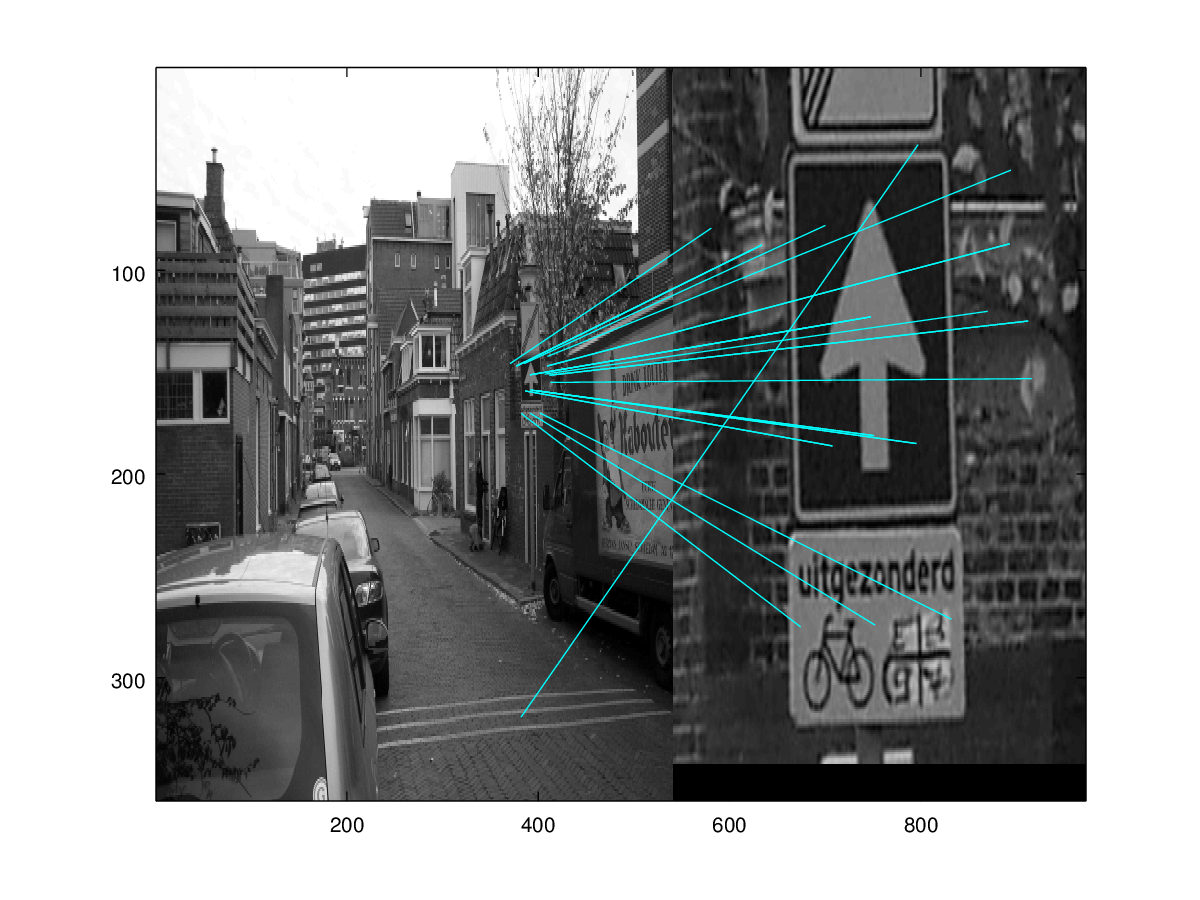
\includegraphics[width=0.45\textwidth]{./img/street-d1-match.png} & 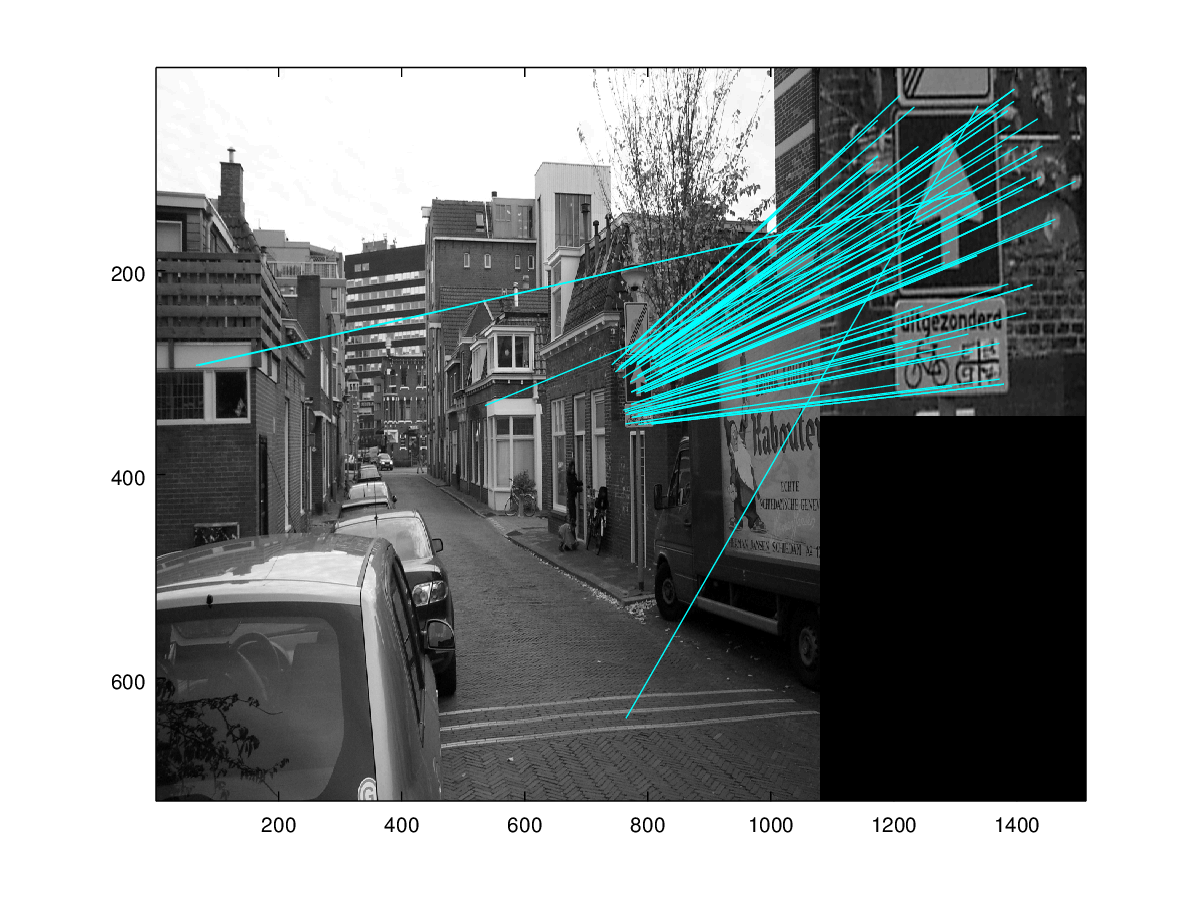
\includegraphics[width=0.45\textwidth]{./img/streetlarge-d1-match.png} \\
    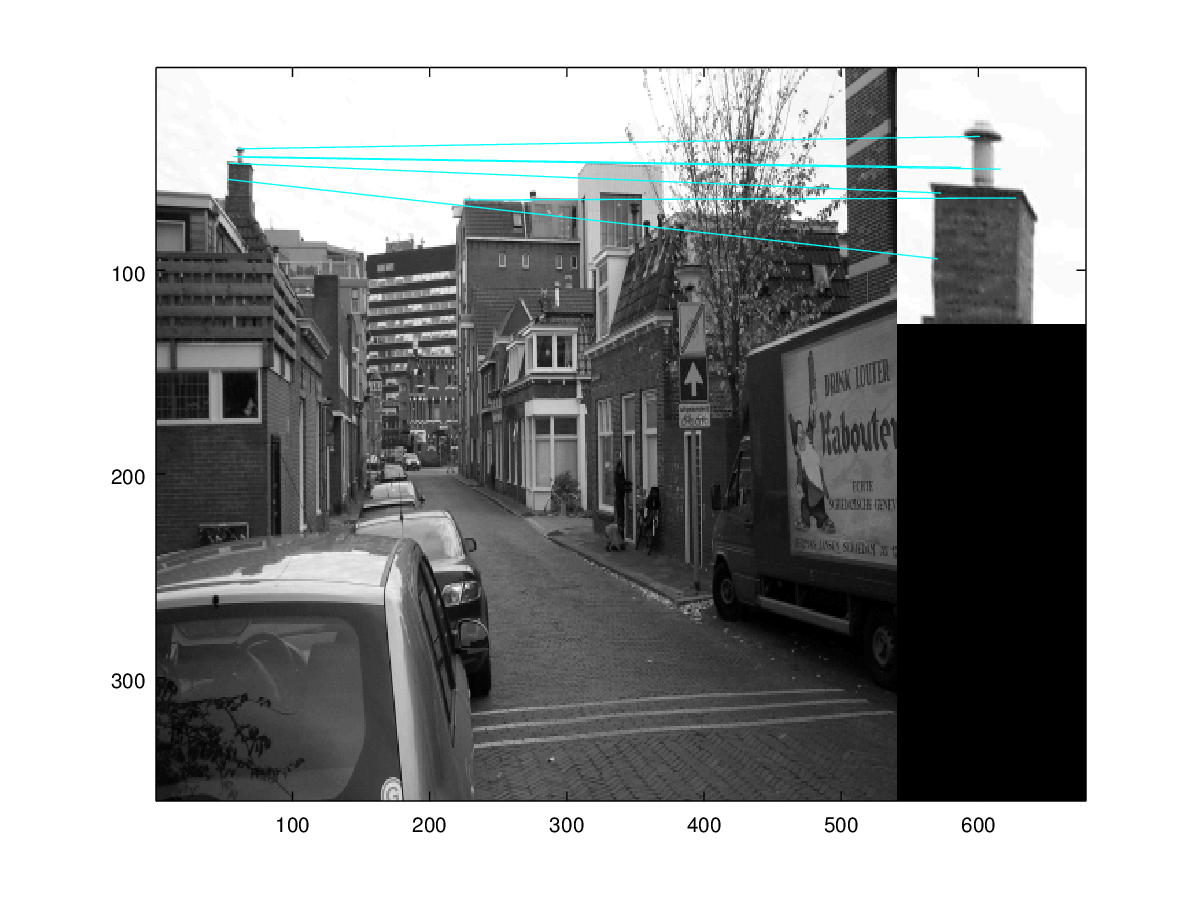
\includegraphics[width=0.45\textwidth]{./img/street-d2-match.png} & 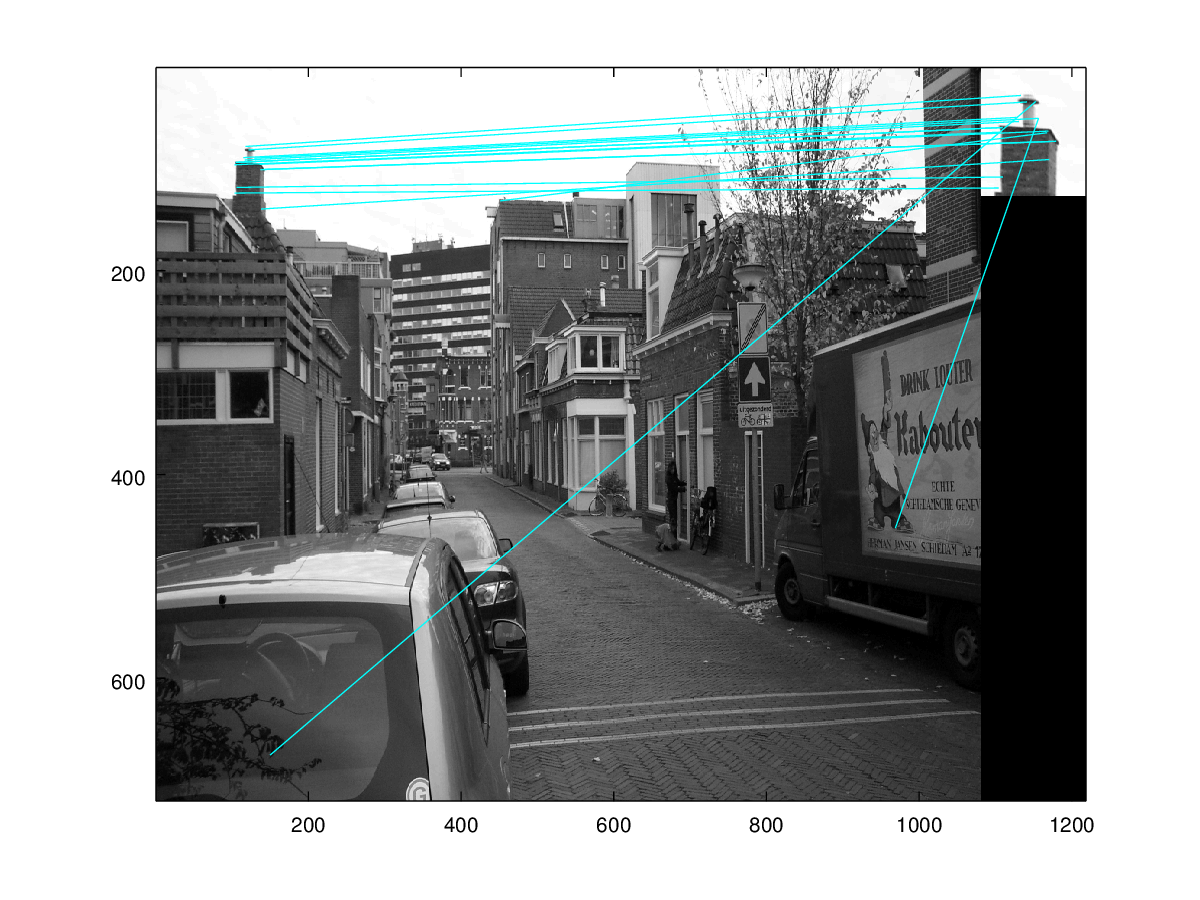
\includegraphics[width=0.45\textwidth]{./img/streetlarge-d2-match.png} \\
    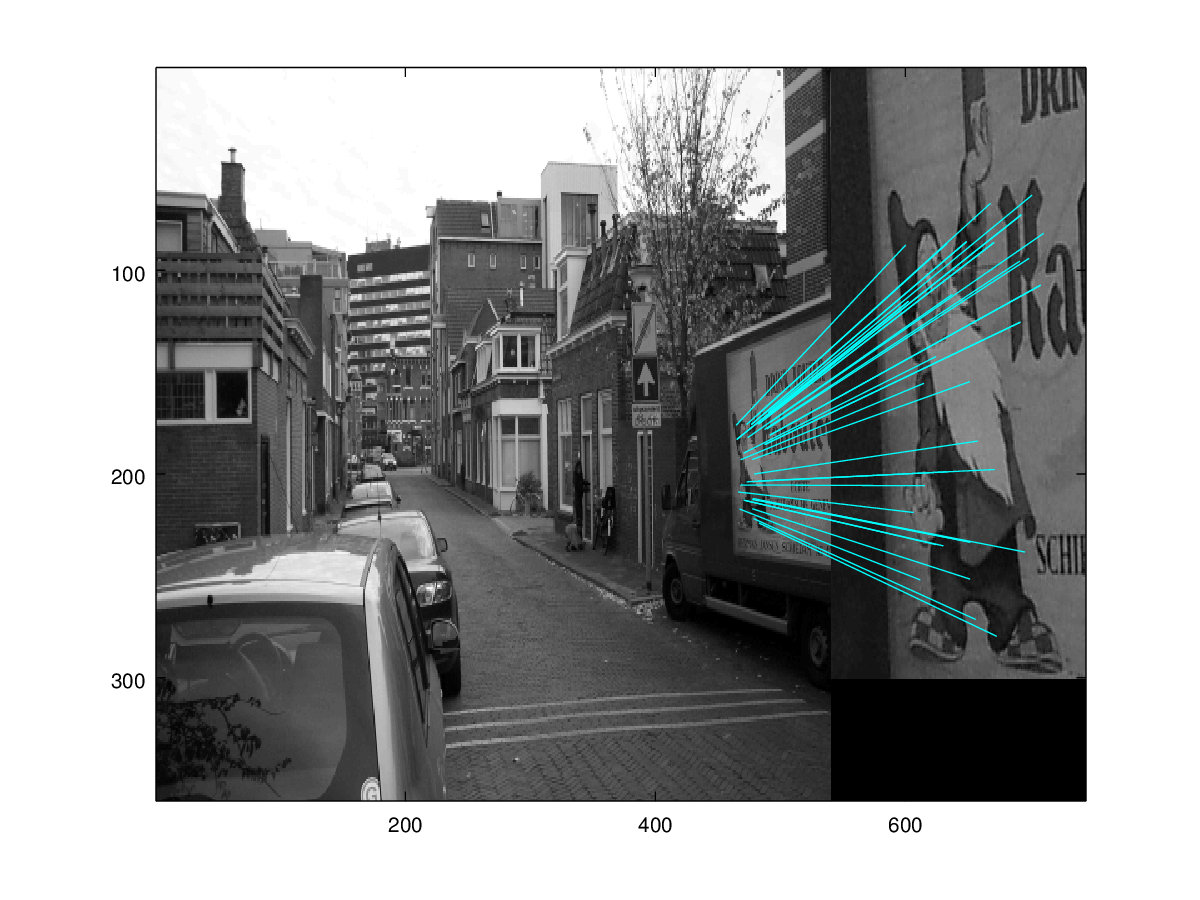
\includegraphics[width=0.45\textwidth]{./img/street-d3-match.png} & 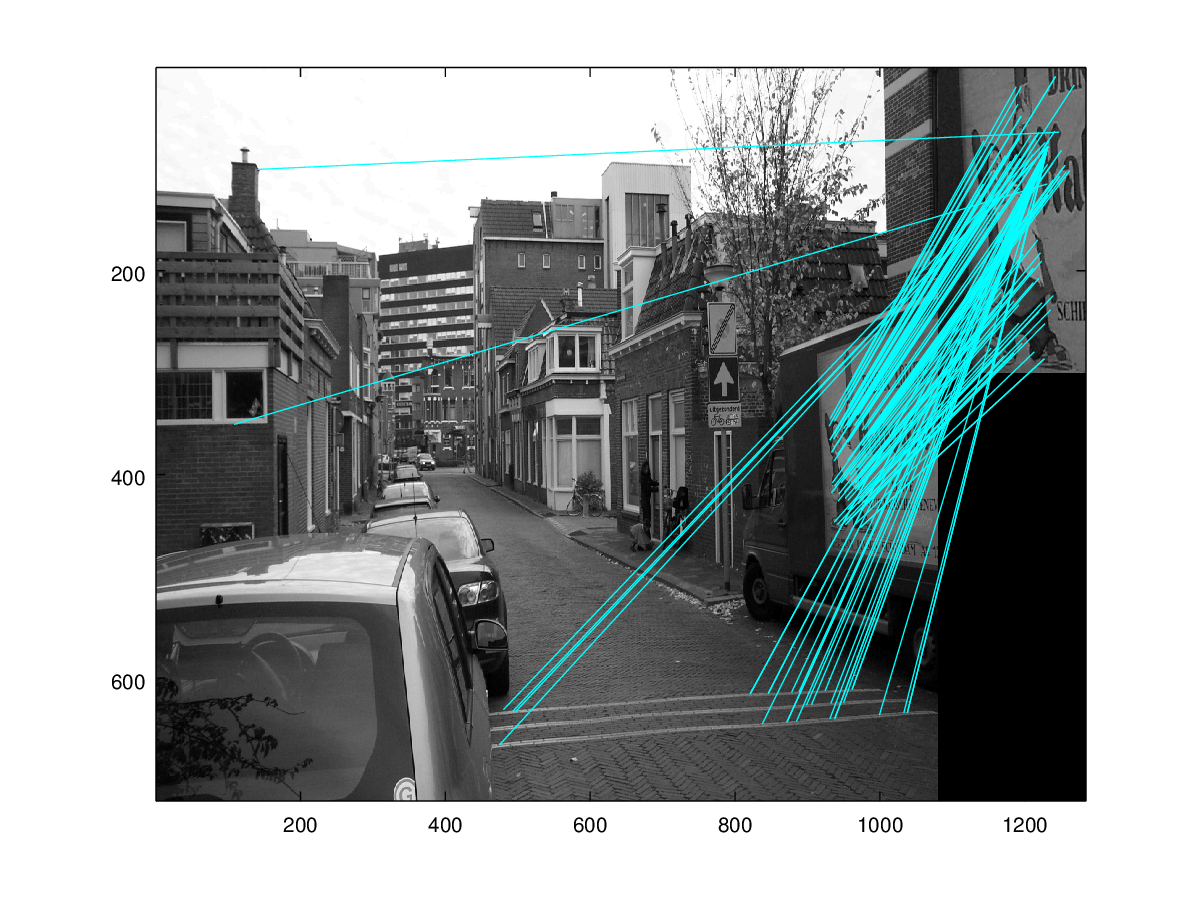
\includegraphics[width=0.45\textwidth]{./img/streetlarge-d3-match.png} \\
    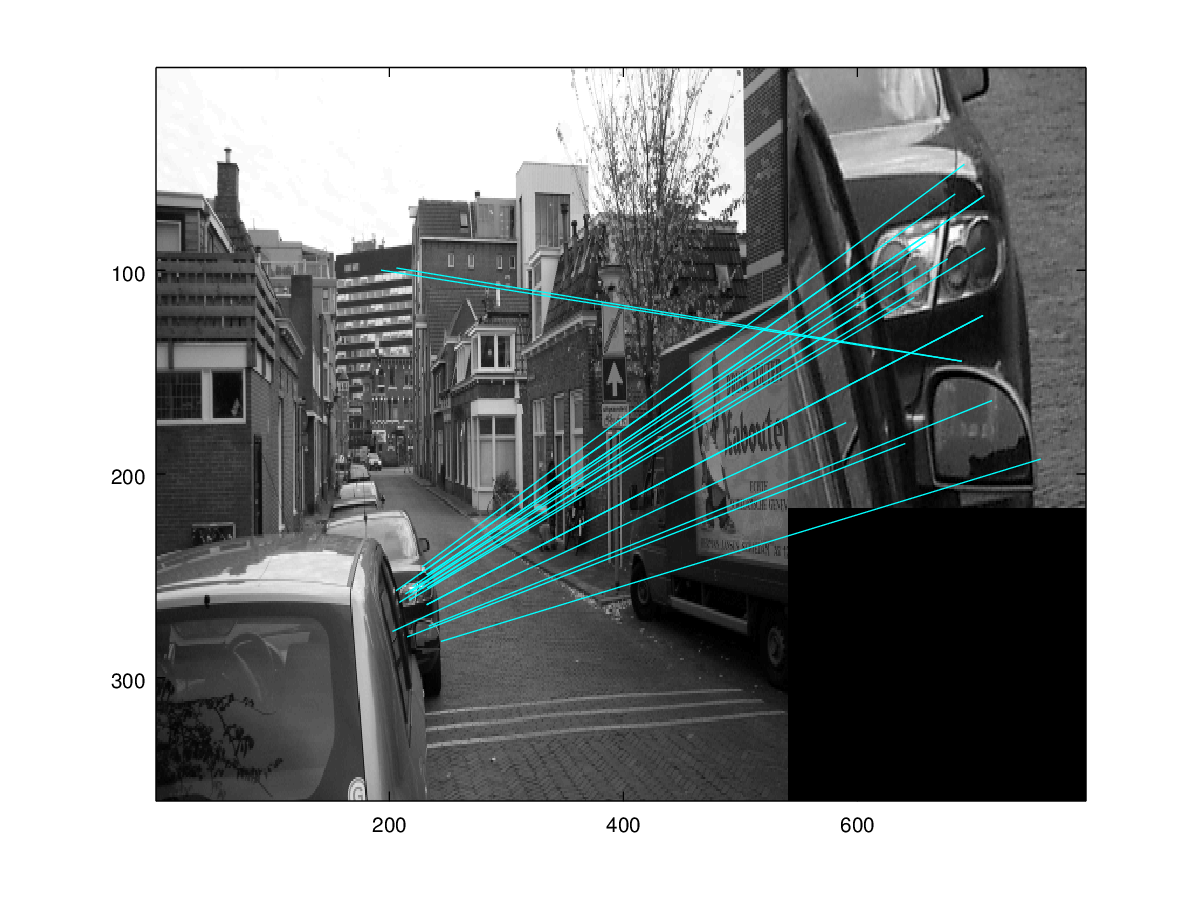
\includegraphics[width=0.45\textwidth]{./img/street-d4-match.png} & 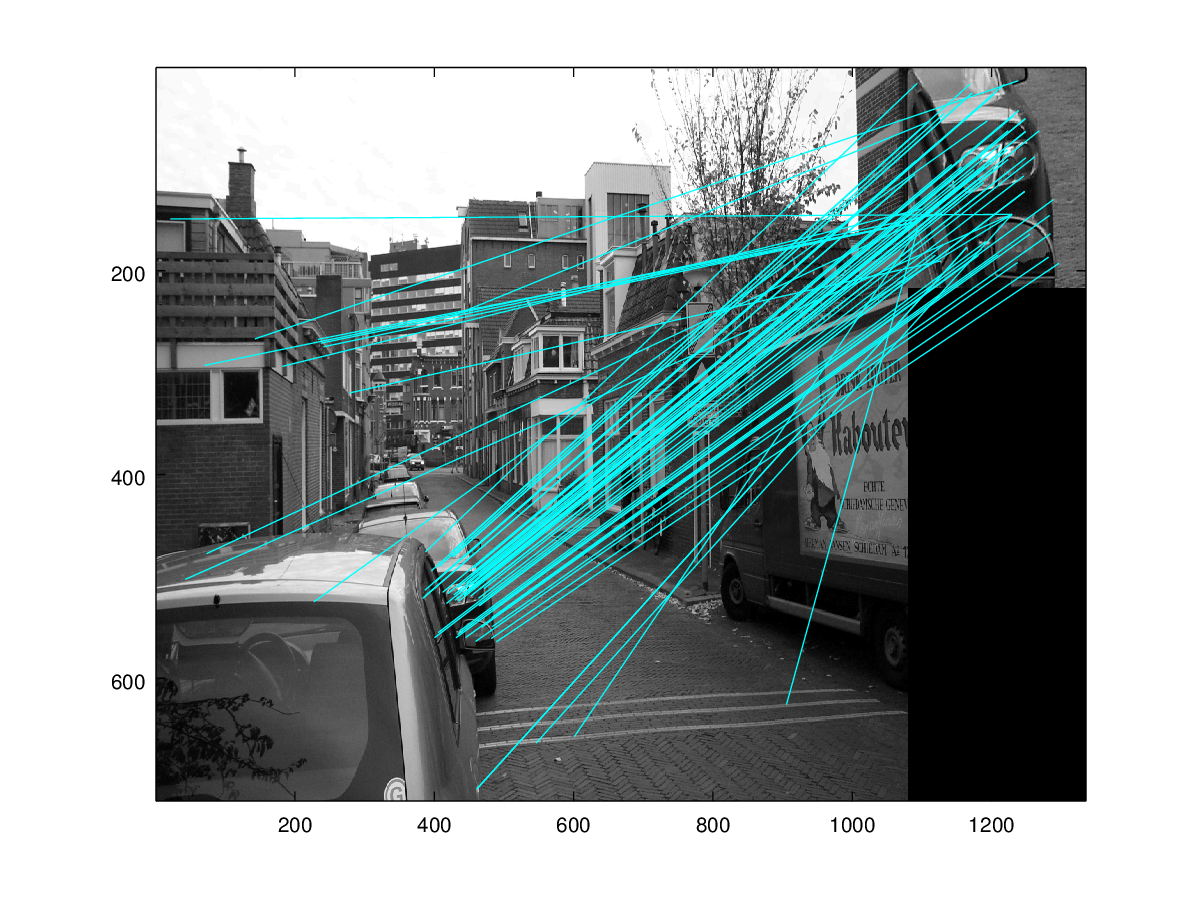
\includegraphics[width=0.45\textwidth]{./img/streetlarge-d4-match.png} \\
\end{tabular}
\caption{The SIFT matches of the street and large street scene with the detail 1 to 4 vertically images.}
\label{fig:streetdetails14}
\end{figure}

Let us consider the effect of the resolution of the scene images with respect to the matched objects.
Figure \ref{fig:streetdetails14} and \ref{fig:streetdetails5} show the results of SIFT matching.
As can be seen in the images the number of matches is higher, but the number of mismatches also increased.
If we ignore the mismatches for now, then we get that the number of matches increased approximately linearly with the number of keys in the scene image.
Table \ref{tab:streetdetails} shows the number of matches per image combination, while Table \ref{tab:streetkeys} lists the number of keys per image.
In this case the large image has about 3 to 4 times the amount of keys with respect to the normal image and the number of matches increased with a similar factor.

\begin{figure}
\centering
\begin{tabular}{c}
    Normal street image \\
    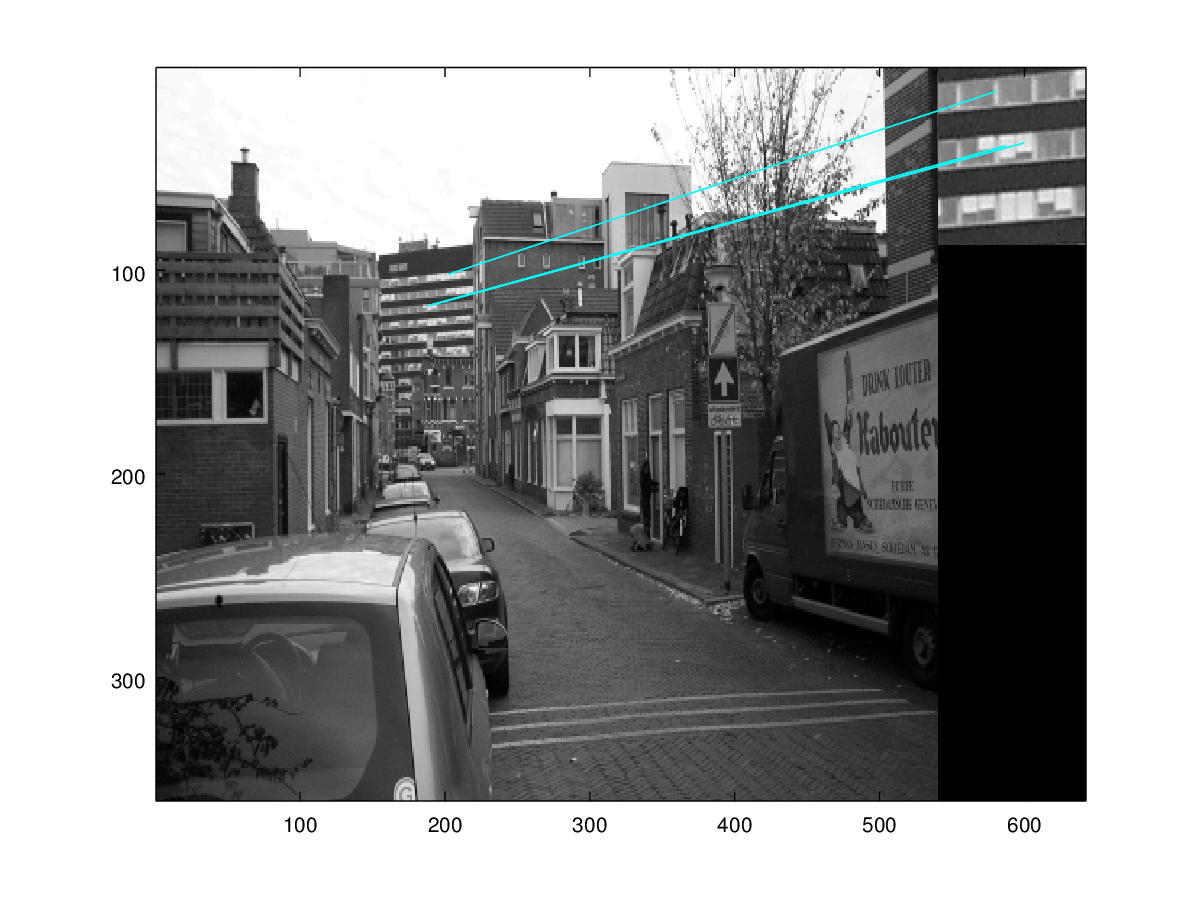
\includegraphics[width=0.9\textwidth]{./img/street-d5-match.png} \\
    Large street image \\
    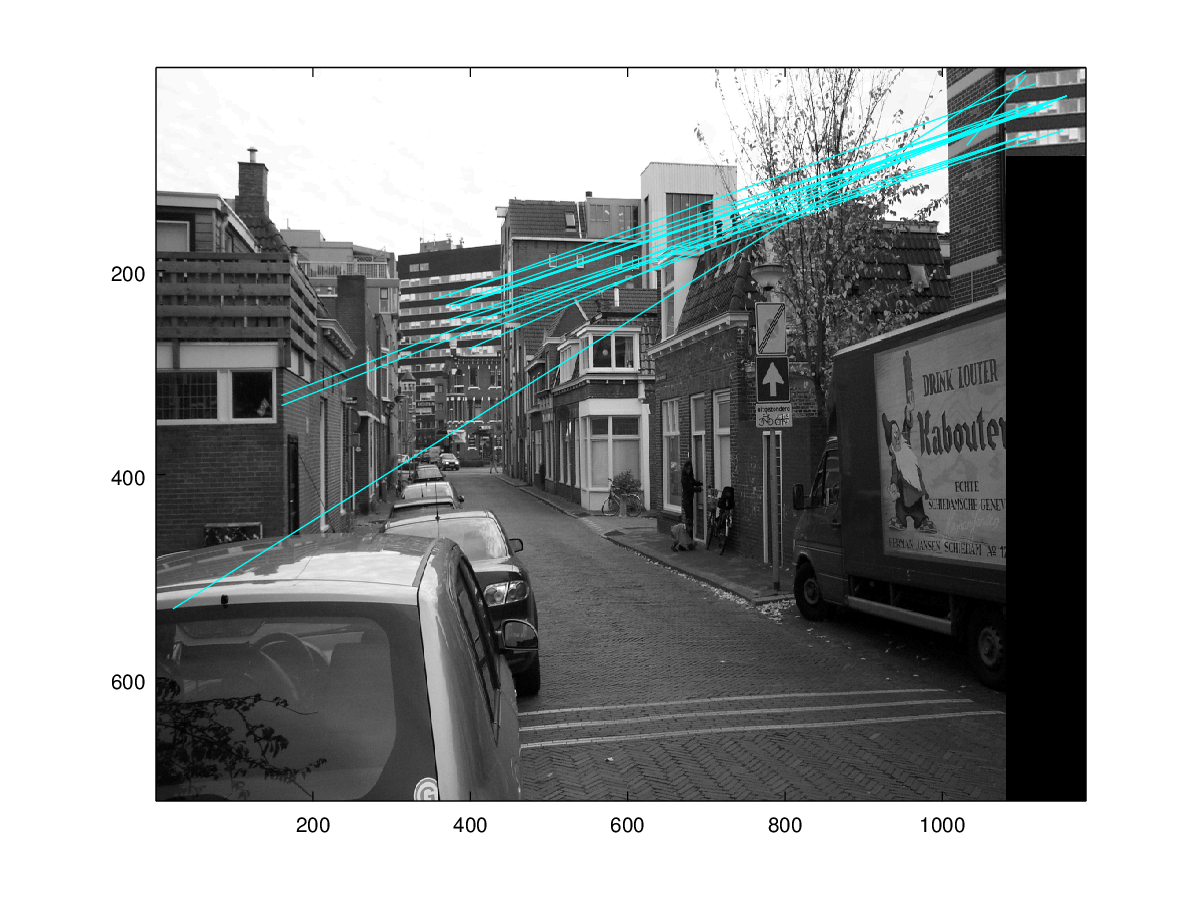
\includegraphics[width=0.9\textwidth]{./img/streetlarge-d5-match.png} \\
\end{tabular}
\caption{The SIFT matches of the street and large street scene with the detail 5 image.}
\label{fig:streetdetails5}
\end{figure}

The number of mismatches seems to be related to the number of keys of the object relative to the number of keys of the scene.
This is mainly based on the observation that in Figure \ref{fig:streetdetails14} and \ref{fig:streetdetails5} the larger street image seems to have more mismatches.
Object images that are about have the size of the scene image seem to do ok, but smaller ones have plenty of mismatches.
The extreme case is detail image 5 with the large street image, most of the matches are mismatches.
So having higher resolution one one image does not decrease the number of mismatches.

\begin{table}
    \centering
    \begin{tabular}{c|c|c|c|c|c|c}
        Street & Large street & Detail 1 & Detail 2 & Detail 3 & Detail 4 & Detail 5 \\
        \hline
        1452 & 5216 & 1592 & 46 & 588 & 368 & 126 \\
    \end{tabular}
    \caption{The number of keys per image.}
    \label{tab:streetkeys}
\end{table}

\begin{table}
    \centering
    \begin{tabular}{l|r|r|r|r|r|}
        & detail 1 & detail 2 & detail 3 & detail 4 & detail 5 \\
        \hline
        Street & 25 & 6 & 37 & 20 & 6 \\
        \hline
        Large street & 82 & 17 & 110 & 73 & 17 \\
        \hline
    \end{tabular}
    \caption{The number of matches between the different street scenes.}
    \label{tab:streetdetails}
\end{table}

\section*{Exercise 2}
Matching the detail images from the street scene with the scene from David Lowe and vice-versa yields a low number of matches.
This is expected, because the detail images should not be present in the source image. The number of matches can be seen in Table \ref{tab:mismatches}.
\begin{table}[H]
	\centering
	\begin{tabular}{l|l|r}
		Source image & detail image & Number of matches\\
		\hline
		scene & detail1 & 1\\
		scene & detail2 & 0\\
		scene & detail3 & 0\\
		scene & detail4 & 2\\
		scene & detail5 & 0\\
		street & basmati & 1\\
		street & book & 1\\
		street & box & 2
	\end{tabular}
	\caption{Number of matches using Sift on detail images not present in the source image}
	\label{tab:mismatches}
\end{table}
%TODO: Jan, kun jij hier nog een vergelijking schrijven met een goede match?
\noindent The number of matches is small with a detail image not present, compared to the number of matches on a detail image that is present. Therefor a low percentage based threshold can be used to claim a real match. 

\section*{Exercise 3}

\section*{Exercise 4}
%TODO: Jan, kun jij hier misschien nog de juiste verwijzingen naar de afbeeldingen toevoegen?
The detail book image Figure \ref{missing} is sheared and compared to the orignal scene image from Figure \ref{missing}.
The number of matches with different shear values can be seen in Table \ref{tab:sheared}.
\begin{table}[H]
	\centering
	\begin{tabular}{l|r}
		Shear amount  & Number of matches\\
		\hline
		0 pixels & 98\\
		25 pixels & 100\\
		50 pixels & 91\\
		100 pixels & 42\\
		200 pixels & 3\\
		300 pixels & 0\\
		400 pixels & 0
	\end{tabular}
	\caption{Number of matches using Sift on detail sheared detail images present in the source image}
	\label{tab:sheared}
\end{table}
\noindent Up to 50 pixels of shear still yields a similar amount of matches compared to the original detail image.
Higher values yield a significantly lower number of matches. Therefor it seems that Sift is not shear invariant.\\

\noindent The amount of shear which still yields tollarable results might depent on the size of the detail image. A shear of 100 pixels is almost a third of the original width of the image.

%TODO: ik weet niet of er nog meer bij kan, maar dit lijkt me het punt wat hij wil bereiken.

\end{document}
